\section{Introduction}

\subsection{Preface}
\texttt{PyCorrFit} was written to simplify the work with experimentally obtained correlation curves. These can be processed independently (operating system, location, hour of the day). PyCorrFit supports commonly used file formats and enables users to allocate and organize their data in a simple way.\\

\noindent PyCorrFit is free software: you can redistribute it and/or modify it
under the terms of the GNU General Public License as published 
by the Free Software Foundation, either version 2 of the License, 
or (at your option) any later version\footnote{\url{http://www.gnu.org/licenses/gpl.html}}.

\subsubsection*{What PyCorrFit can do}
\begin{itemize}
\item Load correlation curves from numerous correlators
\item Process these curves (e.g. background correction, s. Tools section \ref{sec:tools} )
\item Fit a model function (many included) to an experimental curve
\item Import user defined models for fitting
\item Many batch processing features
\item Save/load entire PyCorrFit sessions
\end{itemize}

\subsubsection*{What PyCorrFit is not}
\begin{itemize}
\item A multiple-$\tau$ correlator
\item A software to operate hardware correlators
\end{itemize}

\subsection{System prerequisites}
\subsubsection{Hardware}
This documentation addresses the processing of correlation curves with PyCorrFit. {PyCorrFit} was successfully used with the following setups:
\begin{itemize}
\item[1.]
     APD: Photon Counting Device from PerkinElmer Optoelectronics, Model: 	 \texttt{SPCM-CD3017}\\
     Correlator: Flex02-01D/C from correlator.com with the shipped software 	
	    		 \texttt{flex02-1dc.exe}.
\item[2.]
    APD: Photon Counting Device from PerkinElmer Optoelectronics\\
    Correlator: ALV-6000
\item[3.] LSM Confocor2 or Confocor3 setups from Zeiss, Germany.
\end{itemize}

\subsubsection{Software}
\label{cha:soft}
The latest version of PyCorrFit can be obtained from the internet via \url{http://fcstools.dyndns.org/pycorrfit/}.
\begin{itemize}
\item \textbf{Windows}.
For Windows XP or Windows 7, stand-alone binary executables are available from the download page. 
\item \textbf{Linux}.
There are executable binaries for widely used distributions (e.g. Ubuntu).
\item \textbf{Sources}
The program was written in Python, keeping the concept of cross-platform programming in mind. To run PyCorrFit on any other operating system, the installation of Python v.2.6.5 is needed. Furthermore, the following additional python modules are required:\\
\texttt{\\
python-matplotlib ($\geq$ 1.0.1) \\
python-numpy ($\geq$ 1.5.1) \\
python-scipy ($\geq$ 0.8.0) \\
python-sympy ($\geq$ 0.7.1) \\
python-yaml \\
python-wxtools \\
python-wxgtk2.8-dbg \\
}
\\
For older versions of Ubuntu, some of the above package versions are not listed in the package repository. To enable the use of PyCorrFit on those systems, the following tasks have to be performed:
\begin{itemize}
\item[ ] \textbf{matplotlib}. The tukss-ppa includes version 1.0.1. After adding the repository (\texttt{apt-add-repository ppa:tukss/ppa}), matplotlib can be installed as usual.
\item[ ] \textbf{numpy}. The package from a later version of Ubuntu can be installed: \url{https://launchpad.net/ubuntu/+source/python-numpy/}
\item[ ] \textbf{scipy}. The package from a later version of Ubuntu can be installed: \url{https://launchpad.net/ubuntu/+source/python-scipy/}
\item[ ] \textbf{sympy}. To enable importing external model functions, sympy is required. It is available from \url{http://code.google.com/p/sympy/downloads/list}. Unpacking the archive and executing \texttt{python setup.py install} within the unpacked directory will install sympy.
\end{itemize}
\end{itemize}

\noindent \textbf{\LaTeX}.
PyCorrFit can save correlation curves as images using matplotlib. It is also possible to utilize Latex to generate these plots. On Windows, installing MiKTeX  with ``automatic package download'' will enable this feature. On other systems, the packages LaTeX, dvipng, Ghostscript and the scientific latex packages texlive-science and texlive-math-extra need to be installed.


\section{Theoretical background}


\subsection{Derivation of FCS model functions}
This section introduces the calculation of FCS model functions. It supplies some background information and points out general properties of correlation functions.
	
	\subsubsection{General Autocorrelation function for a single species}
	FCS model functions describe how the signal $F(t)$, emitted from a certain observation volume, is temporally dependent on its own past (autocorrelation) or on some other signal (cross-correlation). The autocorrelation $G(\tau)$ of a signal $F(t)$ is computed as follows:
	\newline
	\newline
	%\fbox{ {
	\begin{minipage}{\textwidth}
	%\textbf{Mathematical foundation - Autocorrelation function:}
	\begin{equation}
	G(\tau) = \frac{\langle \delta F(t) \delta F(t+\tau) \rangle}{\langle F(t) \rangle^2} = \frac{g(\tau)}{\langle F(t) \rangle^2}.
	\end{equation}
	\begin{itemize} \small
	\item[$G(\tau)$] normalized autocorrelation curve
	\item[$\tau$] lag time
	\item[$\langle F \rangle$] the expectation value of $F(t)$. Applying the ergodic theorem, this can be rewritten as the time average \[ \langle F(t) \rangle = \lim_{T \rightarrow \inf }\frac{1}{T} \int_0^T F(t) \mathrm{d}t. \]	
	\item[$\delta F(t)$] $= F(t) - \langle F(t) \rangle$
	\item[$g(\tau)$] non normalized autocorrelation curve
	\end{itemize}
	\end{minipage}
	%} 
	%}
	\newline
	\newline
	\newline
	The Fluorescence signal is dependent on the size and shape of the detection volume (e.g. Gaussian shaped for confocal setups or exponential decaying for TIRF setups), on the propagator of the diffusing dye (free diffusion, diffusion with flow, etc.) and the brightness and concentration of the dye under observation.  \\
	\newline
	%\fbox{ {
	\begin{minipage}{\textwidth}
	%\textbf{General Correlation function for a single species:}
	\begin{equation}
	G(\tau) = \frac{  q^2 C \int \! \mathrm{d}^3 r \int \! \mathrm{d}^3 r'  \, \Omega(\mathbf{r})\Phi(\mathbf{r}, \mathbf{r'}, \tau) \Omega(\mathbf{r'})  }{\langle F(t) \rangle^2}
	\end{equation}
	\begin{itemize} \small
	\item[$q$] molecular brightness, dependent on quantum yields, absorption cross sections, detection efficiencies and excitation intensity.
	\item[$\Omega$] 3D molecule detection function, dependent on point spread function (PSF), shape of pinholes used for detection, excitation laser profile.
	\item[$\Phi$] diffusion propagator. The distribution of dyes in a liquid follows Fick's laws of diffusion. For free diffusion, this is a simple Gaussian distribution.
	\item[$F$] fluorescence signal of the sample. It is defined as
	\[ F(t) = q \int \! \mathrm{d}^3 r \, \Omega(\mathbf{r}) c(\mathbf{r}, t) \] with $c(\mathbf{r}, t)$ being dye distribution (particle concentration) inside the detection volume.
		\item[$C$] average concentration of the dye following the dynamics of the propagator $\Phi$. Using the ergodic hypothesis and assuming a normalized molecule detection function $\Omega$, $ C = \langle F(t) \rangle / q $.
	\end{itemize}
	\end{minipage}
	%} 
	%}
	
	
	\subsubsection{General Autocorrelation function for multiple species}
	Most experiments do not only include a single species of fluorescent dye. When considering a three dimensional detection volume with a freely diffusing dye, adding a lipid bilayer with a different fluorescent dye (diffusing in two dimensions inside the bilayer) will result in two distinct contributions to the fluorescence signal, namely 2D diffusion and 3D diffusion. For $n$ different species inside the detection volume, the autocorrelation function becomes:
	\newline
	\newline
	%\fbox{ {
	\begin{minipage}{\textwidth}
	%\textbf{General Correlation function for n species:}
	\begin{equation}
	G(\tau) = \frac{g(\tau)}{\langle F(t) \rangle^2} =  \frac{\sum_{i=1}^n \sum_{j=1}^n g_{ij}(\tau)}{\langle F(t) \rangle^2}
	\end{equation}
	\begin{equation}
	g_{ij}(\tau) = q_i q_j \int \! \mathrm{d}^3 r \int \! \mathrm{d}^3 r'  \, \Omega(\mathbf{r})\Phi_{ij}(\mathbf{r}, \mathbf{r'}, \tau) \Omega(\mathbf{r'})  
	\end{equation}
	\begin{itemize} \small
	\item[$g(\tau)$] non normalized correlation function
	\item[$g_{ij}(\tau)$] non normalized cross correlation between two species $i$ and $j$
	\item[$q_i$] molecular brightness of species $i$
	\item[$\Omega$] 3D molecule detection function
	\item[$\Phi_{ij}$] diffusion propagator computed from species $i$ with species $j$. If species $i$ and $j$ are independently diffusing, then $\Phi_{ij}$ is zero. 
	$ C_{ij} \Phi_{ij}(\mathbf{r}, \mathbf{r'}, \tau) = \, \langle \delta c_i(\mathbf{r},0) \delta c_j(\mathbf{r'}, \tau) \rangle $ 
	\item[$C_{ij}$] average concentration of objects following the dynamics of $\Phi_{ij}$. If $i=j$, $C_{ii}=C_i$ is the concentration of the dye $i$.
	\end{itemize}
	\end{minipage}
	%} 
	%}
	\newline
	\newline
	If the propagators $\Phi_{ij}(x,y,z; x',y',z'; \tau)$ and the molecule detection function $\Omega(x,y,z)$ factorize into an axial ($z$) and a lateral ($x,y$) part, so will $g_{ij}(\tau)$:
	\begin{equation}
	g_{ij}(\tau) = q_i q_j \cdot g_{ij,z}(\tau) \cdot g_{ij,xy}(\tau)
	\end{equation}
	Following the example with a freely diffusing species $A$ and a laterally diffusing species $B$ inside a membrane at $z = z_0$, it can be concluded:
	\begin{eqnarray*}
	g_{AA}(\tau) = && q_A^2 \cdot g_{AA,z}(\tau) \cdot g_{AA,xy}(\tau) \\
	g_{BB}(\tau) = && q_B^2 \cdot g_{BB,z_0}(\tau) \cdot g_{BB,xy}(\tau) \\
	g_{AB}(\tau) = g_{BA} (\tau) = && q_A q_B \cdot g_{AB,z}(\tau) \cdot g_{AB,xy}(\tau)  \\
	g(\tau) = && g_{AA}(\tau) + 2 g_{AB}(\tau) + g_{BB}(\tau)
	\end{eqnarray*}
	To obtain the normalized autocorrelation function, the average $\langle F(t) \rangle$ has to be calculated:
	\begin{eqnarray*}
	F(t) = && \sum_{i=1}^n F_i(t) \\
	F_A(t) = && q_A \int \! \mathrm{d}^3 r \, \Omega(\mathbf{r}) C_A(\mathbf{r}, t) \\
	F_B(t) = && q_B \int \! \mathrm{d}x \! \int \! \mathrm{d}y \, \Omega(x,y,z=z_0) C_B(x,y, t)  \\
	\langle F(t) \rangle = && \langle F_A(t) \rangle + \langle F_B(t) \rangle
	\end{eqnarray*}
	It is noticeable, that $C_B$ is a 2D concentration, whereas $C_A$ is a 3D concentration. Since there is no correlation between the two freely diffusing species $A$ and $B$, $g_{AB}(\tau)$ is zero. The normalized autocorrelation curve may now be calculated like this:
	\begin{eqnarray*}
	G(\tau) = && \frac{g(\tau)}{\langle F(t) \rangle^2} \\
	G(\tau) = && \frac{g_{AA}(\tau) + g_{BB}(\tau)}{(\langle F_A(t) \rangle + \langle F_B(t) \rangle)^2} \\
	\end{eqnarray*}

	\subsubsection{Cross-correlation}
	Cross-correlation is a generalization of autocorrelation. Cross-correlation functions are derived in the same manner as autocorrelation functions. Here, two signals are cross-correlated to obtain the correlation function.
	\begin{equation}
	G_{XY}(\tau) = \frac{\langle \delta F_X(t) \delta F_Y(t+\tau) \rangle}{\langle F_X(t) \rangle \langle F_Y(t) \rangle}
	\end{equation}
	
	
	\subsubsection{Extension of the theory}
	By modifying the propagator $\Phi$ and the detection volume $\Omega$, other effects, like triplet blinking or binding reactions can be quantified. In many cases, analytical solutions to the above integrals can not be found and approximations have to be made. The Gaussian shaped detection profile in confocal FCS is already an approximation. However, it is close to the real shape and deviations from the true results are considered to be small \cite{Zhang2007}.


\subsection{Non-linear least squares fit}
\label{cha:PyCorFit_leastsq}
PyCorrFit uses the non-linear least squares fitting capabilities from \texttt{scipy.optimize}. This package utilizes the Levenberg–Marquardt algorithm to minimize the sum of the squares. More information on this topic can be obtained from the online documentation of \texttt{leastsq}\footnote{\url{http://docs.scipy.org/doc/scipy/reference/generated/scipy.optimize.leastsq.html##scipy.optimize.leastsq}}. 
One can define a distance $d(G,H)$ between two discrete functions $G$ and $H$ with the discrete domain of definition $\tau_1 \dots \tau_n$ as the sum of squares:
\begin{equation}
d(G,H) = \sum_{i=1}^n \left[ G(\tau_i) - H(\tau_i) \right]^2
\end{equation}
The least squares method minimizes this distance between the model function $G$ and the experimental values $H$ by modifying $k$ additional fitting parameters $\alpha_1, \dots, \alpha_k$:
\begin{equation}
\chi^2 = \min_{\alpha_1, \dots, \alpha_k} \sum_{i=1}^n \left[ G(\tau_i,\alpha_1, \dots, \alpha_k) - H(\tau_i) \right]^2
\end{equation}
The minimum distance $\chi^2$ is used to characterize the success of a fit. Note, that if the number of fitting parameters $k$ becomes too large, multiple values for $\chi^2$ can be found, depending on the starting values of the $k$ parameters.


\subsection{Weighted fitting}
In certain cases, it is useful to implement weights $\sigma_i$ for the calculation of $\chi^2$. For example, very noisy parts of a correlation curve can falsify the resulting fit. In PyCorrFit, weighting is implemented as follows:
\begin{equation}
\chi^2_\mathrm{weighted} = \min_{\alpha_1, \dots, \alpha_k} \sum_{i=1}^n  \frac{\left[ G(\tau_i,\alpha_1, \dots, \alpha_k) - H(\tau_i) \right]^2}{\sigma_i}
\end{equation}
PyCorrFit uses different approaches to calculate the weights $\sigma_i$ from the experimental data. The different approaches to calculate the weights implemented in PyCorrFit are explained in \hyref{section}{cha_graphint}.



\section{Working with PyCorrFit}
\subsection{Data file formats}
\label{sec:fileformats}
PyCorrFit supports numerous data file formats. If a file format is not listed here, there are two options to make them work with PyCorrFit:
\begin{itemize}
\item[-] Conversion to the native PyCorrFit \mytilde .csv file format.
\item[-] Implementation of the file format within the \texttt{readfiles} module of PyCorrFit. \texttt{\_\_init\_\_.py} has to be edited and a script \texttt{read\_FileFormat.py} has to be added.
\end{itemize}

Supported file formats:
\begin{itemize}
\item[] \textbf{\mytilde .asc files} are created by e.g. the ALV-6000 hardware correlator.
\item[] \textbf{\mytilde .csv files} are the native PyCorrFit data files. See \ref{text:csv} for more information.
\item[] \textbf{\mytilde .fcs files} are created by some ConfoCor setups (e.g. AIM 4.2).
\item[] \textbf{\mytilde .mat files} are files generated by a Matlab program written by Jonas Ries. This was implemented for convenience.
\item[] \textbf{\mytilde .sin files} are created by the Flex correlators from correlator.com.
\item[] \textbf{\mytilde .zip files} may contain any of the files listed here.
\end{itemize}

\subsection{PyCorrFit file formats}
These are file formats that were designed for PyCorrFit.


\subsubsection{.csv data files}
\label{text:csv}
This is the recommended way to store data from FCS experiments. \mytilde .csv files are directly readable by any editor from any platform. There is a certain syntax that has to be followed for \mytilde .csv files to be successfully imported by PyCorrFit:


\begin{itemize}

\item The \textbf{encoding} is preferably UTF-8. However, since no special characters are needed to save experimental data, any encoding might work. New line characters are \texttt{\textbackslash r\textbackslash n} (Windows).

\item \textbf{Comments}: Lines starting with a hash (\texttt{\#}) as well as empty lines or lines containing only white space characters are ignored. Exceptions are the keywords listed below.

\item \textbf{Units}: A \mytilde .csv file may contain one correlation curve, as well as up to two intensity traces. The time unit is seconds and the count rate (intensity) is measured in \SI{}{kHz}. Correlation curves are assumed to be calculated from fluctuations around zero, thus the correlation curve has to decrease to zero at large lag times.

\item The first table inside a \mytilde .csv file contains the \textbf{correlation curve}. The table consists of either two or four columns of comma separated values (plus some tab-stops \texttt{\textbackslash t} added by PyCorrFit for better visualization). The first column contains the lag times in seconds and the second column contains the correlation curve. PyCorrFit also saves fitted curve and residuals in the third and fourth column. This additional information is ignored during file import.

\item \textbf{First trace}: The table containing the correlation curve is considered to have ended as soon as the keyword \texttt{\# BEGIN TRACE} appears at the beginning of a line. Then, the trace will be read, again as comma separated values: first column contains time in seconds and second column contains the corresponding signal in \SI{}{KHz}.

\item The optional \textbf{second trace} is initiated with the keyword \texttt{\# BEGIN SECOND TRACE}.

\item \textbf{AC/CC}: There is another keyword, that describes the type of the curve (autocorrelation or cross-correlation). If a line starts with
	\begin{itemize}
	\item \texttt{\# Data type: Cross-correlation} or
	\item \texttt{\# Data type: Autocorrelation},
	\end{itemize}
the corresponding string \texttt{AC} or \texttt{CC} will be used to identify the curve. If no data type is specified, autocorrelation will be assumed. Curves may be personalized by using: \texttt{\# Data type: Autocorrelation \_A1}, which will result in the identifier \texttt{AC\_A1} during import. This is necessary to distinguish many \mytilde .csv files inside a \mytilde .zip file.

\end{itemize}

\subsubsection{.zip data files} 
\mytilde .zip files are either used as session files or as containers for bundled correlation curves. 
\textbf{\mytilde .fcsfit-session.zip files} are used to store entire PyCorrFit sessions including all parameters and modifications. They can be imported as sessions or as experimental curves. 
\textbf{\mytilde .zip files} are containers for files containing correlation curves.

\subsubsection{.txt model function files} 
In addition to the built-in model functions, PyCorrFit supports the import of user defined model functions for fitting. To get started quickly, it is helpful to take a look at some examples online\footnote{``PyCorrFit external model functions'' in the download section at \url{http://fcstools.dyndns.org/pycorrfit}} .
File syntax:
\begin{itemize}

\item \textbf{Parameters}: PyCorrFit works with the following dimensional representation. Any other unit has to be derived from these:
	\begin{itemize}
	\item unit of time        : \SI{1}{ms}
	\item  unit of inverse time: \SI{1000}{s^{-1}}
	\item  unit of distance    : \SI{100}{nm}
	\item  unit of diffusion coefficient  : \SI{10}{µm^2s^{-1}}
	\item  unit of inverse area: \SI{100}{µm^{-2}}
	\item  unit of inverse volume : \SI{1000}{µm^{-3}}
	\end{itemize}


\item The \textbf{encoding} is UTF-8. On Windows, \texttt{Notepad++} can be used. Under Linux, editors like \texttt{gedit} or \texttt{kate} can be used. 


\item \textbf{Comments}: Lines starting with a hash (\texttt{\#}) (except the first line) as well as empty lines or lines containing only white space characters are ignored.

\item \textbf{Name}: The first line contians the name of the correlation function, preceded by a hash, e.g.\\ \texttt{ \# AC Gauss test}.

\item \textbf{Definition of parameters} To define parameters used by the model function, they have to be named and given a starting value. Optionally a dimension of the parameter may be added before the equal sign and separated from the parameter name by a white space. The dimension is only displayed by PyCorrFit and not processed, e.g. 
\\ \texttt{D [10 µm²/s] = 200.0}.\\
This is done for all parameters of the model function. Parameters may not start with a \texttt{G} or \texttt{g}. Also, some variables like \texttt{e} or \texttt{pi} are already mapped and must not be used. The parameter \texttt{tau} is reserved for the corresponding lag times (\SI{}{ms}) and may be used freely.

\item \textbf{Placeholders:} Placeholders must start with a lower \texttt{g}, for example \\  \texttt{gTwoD = 1./(1.+D*tau/a**2)}. 

\item \textbf{Correlation function}: The correlation function is identified by the capital letter \texttt{G}: \\
\texttt{G = 1./n * gThrD * gScan * gTrip}
\end{itemize}
\begin{figure}[tp]
\small
% for case sensitiver Verbatim, we need the package fancyvrb
\begin{Verbatim}[frame = single]

# CS-FCS 3D+S+T (Confocal)

# Circular Scanning FCS model function. 3D diffusion + Triplet.

## Definition of parameters:
# First, the parameters and their starting values for the model function
# need to be defined. If the parameter has a unit of measurement, then it 
# may be added separated by a white space before the "=" sign. The starting
# value should be a floating point number. Floating point abbreviations 
# like "1e-3" instead of "0.001" may be used.

# Diffusion coefficient
D [10 µm²/s] = 200.0
# Structural parameter
w = 5.0
# Waist of the lateral detection area
a [100 nm] = 1.0
# Particle number
n = 5.0
# Scan radius
R [100 nm] = 5.0
# Frequency
f [kHz] = 20.0
# Triplet fraction
T = 0.1
# Triplet time
tautrip [ms] = 0.001

# Th user may wish to substitute certain parts of the correlation function
# with other values to keep the formula simple. This can be done by using the
# prefix "g". All common mathematical functions, such as "sqrt()" or "exp()"
# may be used. For convenience, "pi" and "e" are available as well.

gTrip = 1. + T/(1-T)*exp(-tau/tautrip)
gScan = exp(-(R*sin(pi*f*tau))**2/(a**2+D*tau))
gTwoD = 1./(1.+D*tau/a**2)
gOneD = 1./sqrt(1.+D*tau/(w*a)**2)
gThrD = gTwoD * gOneD

# The final line with the correlation function should start with a "G"
# before the "=" sign.

G = 1./n * gThrD * gScan * gTrip

\end{Verbatim}
\mycaption{user defined model function for PyCorrFit}{The working example shows a model function for circular scanning FCS.\label{fig:extxt}}
\end{figure}
\hyref{Figure}{fig:extxt} shows a working example. External models will be imported with internal model function IDs starting at $7000$. Model functions are checked upon import by PyCorrFit. If the model function does not work, it might be a syntax error, or just an error of \texttt{sympy}. Sympy is used to check the model and is still under development. Model functions will be saved upon session saving.


\subsection{The graphical user interface}
\label{cha_graphint}
\label{sec:PyCorrFitUserInterface}
\hyref{Figure}{fig:PyCorrFitMain} shows the main window of PyCorrFit. It contains a menu bar to access all tools, a notebook with tabs, each tab representing a single curve, and a page - the content of the currently selected tab. 
\begin{figure}[h]
\centering
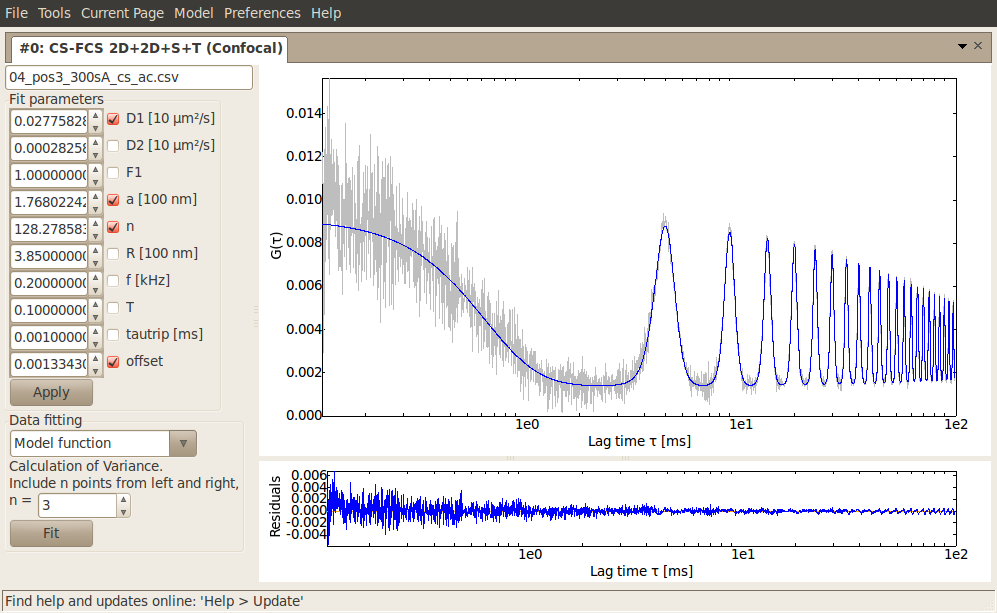
\includegraphics[width=\linewidth]{PyCorrFit_Main.png}
 \mycaption{user interface of PyCorrFit}{A circular scanning FCS (CS-FCS) curve of DiO on a supported lipid bilayer (glass substrate) is shown. The measurement yields a diffusion coefficient of \SI{0.28}{\mu m^2s^{-1}} ($F1=1$, so only one component is fitted). Note that a 2D diffusion model is used and not a 3D model (as shown in \hyref{figure}{fig:extxt}). \label{fig:PyCorrFitMain}}
\end{figure}
\subparagraph*{Page}
Within the page, the user may choose starting parameters for the fitting, select which parameters should be variable during fitting (checked means variable) and select a weighting method. The page displays the experimental and fitted curve, as well as the residuals in the lower plot.

\subparagraph*{Weighting}
Weights can be calculated for each data point using the standard deviation from neighboring points. Since FCS curves naturally have regions where the standard deviation of the experimental data is large (falling inflection points), the standard deviation has to be calculated from curves that mimic the experimental data. The following methods for weighting have been implemented:
\begin{itemize}
\item[] \textbf{Spline}. A spline is fitted to the experimental curve. Weights are calculated from the deviation of the experimental data from the spline. If  the \texttt{Verbose mode} is enabled in  the \texttt{Preferences} menu, the spline fit will be displayed. The number of knots of the spline can be changed by adjusting the number in the dropdown menu. In case of multiple component data, a higher number of knots is required to obtain a fitting spline. For single component data, up to three knots are sufficient.
\item[] \textbf{Model function}. Instead of calculating the weights from a spline, calculate the weights from the previously fitted model function. This method of weighting is iterative - the fit should converge!
\end{itemize}

\subparagraph*{Menus} PyCorrFit is operated through the menu bar. The \texttt{File} menu lets the user load and save files as discussed in section \ref{sec:fileformats}. The \texttt{Tools} menu contains several tools that are described below. The \texttt{Current Page} menu allows the user to perform tasks on the current page. This includes loading experimental data files or saving the currently viewable correlation curve as \mytilde .csv file or as an image. The \texttt{Model} menu lets the user select a model to create a new page. The \texttt{Preferences} menu allows the user to use Latex for plotting (\hyref{section}{cha:soft}) or tells the program to be more verbose (spline fits for calculation of weights will be displayed). The \texttt{Help} menu contains an update function that checks the current program version against the official release of PyCorrFit.

\subsection{Tools}
\label{sec:tools}
The graphical user interface comes with a bunch of tools located in the \texttt{Tools} menu. The \texttt{Tools} menu will become active, once a page is added to the notebook. Each tool opens in a new window. Tools are updated or closed upon change of the current page. All tools are generally self-explanatory:
\begin{itemize}
\item \textbf{Average curves}: Averages experimental curves from all pages, except:
		\begin{itemize}
		\item pages with a different model than the current page,
		\item pages that do not have the same correlation type (autocorrelation or cross-correlation) as the current page,
		\item pages, where the length of the correlation curve does not match the length of the curve of the current page.
		\end{itemize}
		A new page will be created containing the resulting average. The resulting trace is constructed by appending the traces of the averaged curves.
		
\item \textbf{Background correction}: Performs a background correction on the experimental curve. The result is usually a lower particle number after fitting. Backgrounds may be manually set or imported from background measurements (see supported file formats). Background measurements should consist of files containing only one curve and a trace. Else, only the first trace from the first curve will be used.
\begin{equation}
G_\mathrm{corrected}(\tau) = G_\mathrm{measured}(\tau) \cdot \left[ \frac{S}{S-B} \right]^2
\label{eq:BG_correction}
\end{equation}
where $S$ is the average signal of the correlation curve and $B$ is the background signal.
\item \textbf{Batch control}: Perform fitting operations on all pages. Parameters may be imported from other \mytilde .fcsfit-session.zip-files. Application of parameters and fitting of curves is only executed for pages with the same model as the current page.
\item \textbf{Data range selection}: This selects the lag times $\tau$ from the experimental curve that will be displayed. By default, all data from a file will be displayed. 
\item \textbf{Global fitting}: If multiple correlation curves share some of their parameters, a global fit can be applied. Selected correlation curves are added to one array and the squares of the residuals (parametrized curve minus experimental data) are minimized according to the parameters the user chooses within the respective pages. This is useful in two-focus FCS, where two autocorrelation curves and two cross-correlation curves are obtained. These share the parameters particle number $n$ and diffusion time $\tau_{\text{diff}}$. A global fit can be applied such that $n$ and $\tau_{\text{diff}}$ are the same for all curves.
\item \textbf{Slider simulation}: This is useful to visualize the impact of certain parameters on the shape of the correlation function or to set proper starting parameters for a fit.
\item \textbf{Page info}: A most verbose information window that shows all there is to know about the current page. All information that is displayed here will also be saved when exporting a curve as a \mytilde .csv file with the \texttt{Current Page} menu.
\item \textbf{Trace view}: If available, view the trace corresponding to the data of the current page. In case of cross-correlation, two traces will be displayed.
\item  \textbf{Statistics}: Used for large data sets. Save selected parameters (of all pages with the same model as the current page) as a table of tab separated values into one single file.
\end{itemize}
